\documentclass{article}\usepackage[]{graphicx}\usepackage[]{color}
% maxwidth is the original width if it is less than linewidth
% otherwise use linewidth (to make sure the graphics do not exceed the margin)
\makeatletter
\def\maxwidth{ %
  \ifdim\Gin@nat@width>\linewidth
    \linewidth
  \else
    \Gin@nat@width
  \fi
}
\makeatother

\definecolor{fgcolor}{rgb}{0.345, 0.345, 0.345}
\newcommand{\hlnum}[1]{\textcolor[rgb]{0.686,0.059,0.569}{#1}}%
\newcommand{\hlstr}[1]{\textcolor[rgb]{0.192,0.494,0.8}{#1}}%
\newcommand{\hlcom}[1]{\textcolor[rgb]{0.678,0.584,0.686}{\textit{#1}}}%
\newcommand{\hlopt}[1]{\textcolor[rgb]{0,0,0}{#1}}%
\newcommand{\hlstd}[1]{\textcolor[rgb]{0.345,0.345,0.345}{#1}}%
\newcommand{\hlkwa}[1]{\textcolor[rgb]{0.161,0.373,0.58}{\textbf{#1}}}%
\newcommand{\hlkwb}[1]{\textcolor[rgb]{0.69,0.353,0.396}{#1}}%
\newcommand{\hlkwc}[1]{\textcolor[rgb]{0.333,0.667,0.333}{#1}}%
\newcommand{\hlkwd}[1]{\textcolor[rgb]{0.737,0.353,0.396}{\textbf{#1}}}%
\let\hlipl\hlkwb

\usepackage{framed}
\makeatletter
\newenvironment{kframe}{%
 \def\at@end@of@kframe{}%
 \ifinner\ifhmode%
  \def\at@end@of@kframe{\end{minipage}}%
  \begin{minipage}{\columnwidth}%
 \fi\fi%
 \def\FrameCommand##1{\hskip\@totalleftmargin \hskip-\fboxsep
 \colorbox{shadecolor}{##1}\hskip-\fboxsep
     % There is no \\@totalrightmargin, so:
     \hskip-\linewidth \hskip-\@totalleftmargin \hskip\columnwidth}%
 \MakeFramed {\advance\hsize-\width
   \@totalleftmargin\z@ \linewidth\hsize
   \@setminipage}}%
 {\par\unskip\endMakeFramed%
 \at@end@of@kframe}
\makeatother

\definecolor{shadecolor}{rgb}{.97, .97, .97}
\definecolor{messagecolor}{rgb}{0, 0, 0}
\definecolor{warningcolor}{rgb}{1, 0, 1}
\definecolor{errorcolor}{rgb}{1, 0, 0}
\newenvironment{knitrout}{}{} % an empty environment to be redefined in TeX

\usepackage{alltt}

\usepackage[OT4]{polski}
\usepackage[utf8]{inputenc}
\usepackage[T1]{fontenc}
\usepackage[top=2.5cm, bottom=2.5cm, left=2cm, right=2cm]{geometry}
\usepackage{graphicx}
\usepackage{float}
\usepackage[colorlinks=true, linkcolor=blue]{hyperref}
\usepackage{amsmath}
\usepackage{amssymb}



\title{Lista 1}
\author{Mikołaj Langner, Marcin Kostrzewa}
\date{31.3.2021}
\IfFileExists{upquote.sty}{\usepackage{upquote}}{}
\begin{document}

\section{Etap I}

\begin{knitrout}
\definecolor{shadecolor}{rgb}{0.969, 0.969, 0.969}\color{fgcolor}\begin{kframe}
\begin{alltt}
\hlstd{df} \hlkwb{<-} \hlkwd{read.csv}\hlstd{(}\hlstr{'churn.txt'}\hlstd{)}

\hlkwd{dim}\hlstd{(df)}
\end{alltt}
\begin{verbatim}
## [1] 3333   21
\end{verbatim}
\begin{alltt}
\hlkwd{head}\hlstd{(df)}
\end{alltt}
\begin{verbatim}
##   State Account.Length Area.Code    Phone Int.l.Plan VMail.Plan VMail.Message
## 1    KS            128       415 382-4657         no        yes            25
## 2    OH            107       415 371-7191         no        yes            26
## 3    NJ            137       415 358-1921         no         no             0
## 4    OH             84       408 375-9999        yes         no             0
## 5    OK             75       415 330-6626        yes         no             0
## 6    AL            118       510 391-8027        yes         no             0
##   Day.Mins Day.Calls Day.Charge Eve.Mins Eve.Calls Eve.Charge Night.Mins
## 1    265.1       110      45.07    197.4        99      16.78      244.7
## 2    161.6       123      27.47    195.5       103      16.62      254.4
## 3    243.4       114      41.38    121.2       110      10.30      162.6
## 4    299.4        71      50.90     61.9        88       5.26      196.9
## 5    166.7       113      28.34    148.3       122      12.61      186.9
## 6    223.4        98      37.98    220.6       101      18.75      203.9
##   Night.Calls Night.Charge Intl.Mins Intl.Calls Intl.Charge CustServ.Calls
## 1          91        11.01      10.0          3        2.70              1
## 2         103        11.45      13.7          3        3.70              1
## 3         104         7.32      12.2          5        3.29              0
## 4          89         8.86       6.6          7        1.78              2
## 5         121         8.41      10.1          3        2.73              3
## 6         118         9.18       6.3          6        1.70              0
##   Churn.
## 1 False.
## 2 False.
## 3 False.
## 4 False.
## 5 False.
## 6 False.
\end{verbatim}
\begin{alltt}
\hlkwd{str}\hlstd{(df)}
\end{alltt}
\begin{verbatim}
## 'data.frame':	3333 obs. of  21 variables:
##  $ State         : Factor w/ 51 levels "AK","AL","AR",..: 17 36 32 36 37 2 20 25 19 50 ...
##  $ Account.Length: int  128 107 137 84 75 118 121 147 117 141 ...
##  $ Area.Code     : int  415 415 415 408 415 510 510 415 408 415 ...
##  $ Phone         : Factor w/ 3333 levels "327-1058","327-1319",..: 1927 1576 1118 1708 111 2254 1048 81 292 118 ...
##  $ Int.l.Plan    : Factor w/ 2 levels "no","yes": 1 1 1 2 2 2 1 2 1 2 ...
##  $ VMail.Plan    : Factor w/ 2 levels "no","yes": 2 2 1 1 1 1 2 1 1 2 ...
##  $ VMail.Message : int  25 26 0 0 0 0 24 0 0 37 ...
##  $ Day.Mins      : num  265 162 243 299 167 ...
##  $ Day.Calls     : int  110 123 114 71 113 98 88 79 97 84 ...
##  $ Day.Charge    : num  45.1 27.5 41.4 50.9 28.3 ...
##  $ Eve.Mins      : num  197.4 195.5 121.2 61.9 148.3 ...
##  $ Eve.Calls     : int  99 103 110 88 122 101 108 94 80 111 ...
##  $ Eve.Charge    : num  16.78 16.62 10.3 5.26 12.61 ...
##  $ Night.Mins    : num  245 254 163 197 187 ...
##  $ Night.Calls   : int  91 103 104 89 121 118 118 96 90 97 ...
##  $ Night.Charge  : num  11.01 11.45 7.32 8.86 8.41 ...
##  $ Intl.Mins     : num  10 13.7 12.2 6.6 10.1 6.3 7.5 7.1 8.7 11.2 ...
##  $ Intl.Calls    : int  3 3 5 7 3 6 7 6 4 5 ...
##  $ Intl.Charge   : num  2.7 3.7 3.29 1.78 2.73 1.7 2.03 1.92 2.35 3.02 ...
##  $ CustServ.Calls: int  1 1 0 2 3 0 3 0 1 0 ...
##  $ Churn.        : Factor w/ 2 levels "False.","True.": 1 1 1 1 1 1 1 1 1 1 ...
\end{verbatim}
\end{kframe}
\end{knitrout}

\begin{knitrout}
\definecolor{shadecolor}{rgb}{0.969, 0.969, 0.969}\color{fgcolor}\begin{kframe}
\begin{alltt}
\hlstd{df}\hlopt{$}\hlstd{Area.Code} \hlkwb{<-} \hlkwd{as.factor}\hlstd{(df}\hlopt{$}\hlstd{Area.Code)}
\hlstd{df}\hlopt{$}\hlstd{Day.Charge} \hlkwb{<-} \hlkwd{as.integer}\hlstd{(df}\hlopt{$}\hlstd{Day.Charge)}
\end{alltt}
\end{kframe}
\end{knitrout}

\begin{knitrout}
\definecolor{shadecolor}{rgb}{0.969, 0.969, 0.969}\color{fgcolor}\begin{kframe}
\begin{alltt}
\hlkwd{sapply}\hlstd{(df,} \hlkwa{function}\hlstd{(}\hlkwc{x}\hlstd{)} \hlkwd{sum}\hlstd{(}\hlkwd{is.na}\hlstd{(x)))}
\end{alltt}
\begin{verbatim}
##          State Account.Length      Area.Code          Phone     Int.l.Plan 
##              0              0              0              0              0 
##     VMail.Plan  VMail.Message       Day.Mins      Day.Calls     Day.Charge 
##              0              0              0              0              0 
##       Eve.Mins      Eve.Calls     Eve.Charge     Night.Mins    Night.Calls 
##              0              0              0              0              0 
##   Night.Charge      Intl.Mins     Intl.Calls    Intl.Charge CustServ.Calls 
##              0              0              0              0              0 
##         Churn. 
##              0
\end{verbatim}
\end{kframe}
\end{knitrout}

\begin{knitrout}
\definecolor{shadecolor}{rgb}{0.969, 0.969, 0.969}\color{fgcolor}\begin{kframe}
\begin{alltt}
\hlstd{df} \hlkwb{<-} \hlkwd{subset}\hlstd{(df,} \hlkwc{select}\hlstd{=}\hlopt{-}\hlstd{Phone)}
\end{alltt}
\end{kframe}
\end{knitrout}

\begin{knitrout}
\definecolor{shadecolor}{rgb}{0.969, 0.969, 0.969}\color{fgcolor}\begin{kframe}
\begin{alltt}
\hlkwd{sapply}\hlstd{(df[,} \hlkwd{sapply}\hlstd{(df, is.factor)], levels)}
\end{alltt}
\begin{verbatim}
## $State
##  [1] "AK" "AL" "AR" "AZ" "CA" "CO" "CT" "DC" "DE" "FL" "GA" "HI" "IA" "ID" "IL"
## [16] "IN" "KS" "KY" "LA" "MA" "MD" "ME" "MI" "MN" "MO" "MS" "MT" "NC" "ND" "NE"
## [31] "NH" "NJ" "NM" "NV" "NY" "OH" "OK" "OR" "PA" "RI" "SC" "SD" "TN" "TX" "UT"
## [46] "VA" "VT" "WA" "WI" "WV" "WY"
## 
## $Area.Code
## [1] "408" "415" "510"
## 
## $Int.l.Plan
## [1] "no"  "yes"
## 
## $VMail.Plan
## [1] "no"  "yes"
## 
## $Churn.
## [1] "False." "True."
\end{verbatim}
\end{kframe}
\end{knitrout}

\begin{knitrout}
\definecolor{shadecolor}{rgb}{0.969, 0.969, 0.969}\color{fgcolor}\begin{kframe}
\begin{alltt}
\hlkwd{summary}\hlstd{(df)}
\end{alltt}
\begin{verbatim}
##      State      Account.Length  Area.Code  Int.l.Plan VMail.Plan
##  WV     : 106   Min.   :  1.0   408: 838   no :3010   no :2411  
##  MN     :  84   1st Qu.: 74.0   415:1655   yes: 323   yes: 922  
##  NY     :  83   Median :101.0   510: 840                        
##  AL     :  80   Mean   :101.1                                   
##  OH     :  78   3rd Qu.:127.0                                   
##  OR     :  78   Max.   :243.0                                   
##  (Other):2824                                                   
##  VMail.Message       Day.Mins       Day.Calls       Day.Charge   
##  Min.   : 0.000   Min.   :  0.0   Min.   :  0.0   Min.   : 0.00  
##  1st Qu.: 0.000   1st Qu.:143.7   1st Qu.: 87.0   1st Qu.:24.00  
##  Median : 0.000   Median :179.4   Median :101.0   Median :30.00  
##  Mean   : 8.099   Mean   :179.8   Mean   :100.4   Mean   :30.07  
##  3rd Qu.:20.000   3rd Qu.:216.4   3rd Qu.:114.0   3rd Qu.:36.00  
##  Max.   :51.000   Max.   :350.8   Max.   :165.0   Max.   :59.00  
##                                                                  
##     Eve.Mins       Eve.Calls       Eve.Charge      Night.Mins   
##  Min.   :  0.0   Min.   :  0.0   Min.   : 0.00   Min.   : 23.2  
##  1st Qu.:166.6   1st Qu.: 87.0   1st Qu.:14.16   1st Qu.:167.0  
##  Median :201.4   Median :100.0   Median :17.12   Median :201.2  
##  Mean   :201.0   Mean   :100.1   Mean   :17.08   Mean   :200.9  
##  3rd Qu.:235.3   3rd Qu.:114.0   3rd Qu.:20.00   3rd Qu.:235.3  
##  Max.   :363.7   Max.   :170.0   Max.   :30.91   Max.   :395.0  
##                                                                 
##   Night.Calls     Night.Charge      Intl.Mins       Intl.Calls    
##  Min.   : 33.0   Min.   : 1.040   Min.   : 0.00   Min.   : 0.000  
##  1st Qu.: 87.0   1st Qu.: 7.520   1st Qu.: 8.50   1st Qu.: 3.000  
##  Median :100.0   Median : 9.050   Median :10.30   Median : 4.000  
##  Mean   :100.1   Mean   : 9.039   Mean   :10.24   Mean   : 4.479  
##  3rd Qu.:113.0   3rd Qu.:10.590   3rd Qu.:12.10   3rd Qu.: 6.000  
##  Max.   :175.0   Max.   :17.770   Max.   :20.00   Max.   :20.000  
##                                                                   
##   Intl.Charge    CustServ.Calls     Churn.    
##  Min.   :0.000   Min.   :0.000   False.:2850  
##  1st Qu.:2.300   1st Qu.:1.000   True. : 483  
##  Median :2.780   Median :1.000                
##  Mean   :2.765   Mean   :1.563                
##  3rd Qu.:3.270   3rd Qu.:2.000                
##  Max.   :5.400   Max.   :9.000                
## 
\end{verbatim}
\end{kframe}
\end{knitrout}

\section{Etap II}

\begin{knitrout}
\definecolor{shadecolor}{rgb}{0.969, 0.969, 0.969}\color{fgcolor}\begin{kframe}


{\ttfamily\noindent\itshape\color{messagecolor}{\#\# Registered S3 method overwritten by 'GGally':\\\#\#\ \  method from\ \  \\\#\#\ \  +.gg\ \  ggplot2}}

{\ttfamily\noindent\itshape\color{messagecolor}{\#\# \\\#\# Attaching package: 'dplyr'}}

{\ttfamily\noindent\itshape\color{messagecolor}{\#\# The following objects are masked from 'package:stats':\\\#\# \\\#\#\ \ \ \  filter, lag}}

{\ttfamily\noindent\itshape\color{messagecolor}{\#\# The following objects are masked from 'package:base':\\\#\# \\\#\#\ \ \ \  intersect, setdiff, setequal, union}}\end{kframe}
\end{knitrout}

\begin{knitrout}
\definecolor{shadecolor}{rgb}{0.969, 0.969, 0.969}\color{fgcolor}\begin{kframe}
\begin{alltt}
\hlstd{factors} \hlkwb{<-} \hlkwd{subset}\hlstd{(df,} \hlkwc{select}\hlstd{=}\hlkwd{sapply}\hlstd{(df, is.factor))}
\hlstd{numerics} \hlkwb{<-} \hlkwd{subset}\hlstd{(df,} \hlkwc{select}\hlstd{=}\hlkwd{sapply}\hlstd{(df,} \hlkwa{function}\hlstd{(}\hlkwc{x}\hlstd{)} \hlopt{!}\hlkwd{is.factor}\hlstd{(x)))}
\end{alltt}
\end{kframe}
\end{knitrout}

\begin{description}


\item{a)}



\item{b)}

\begin{knitrout}
\definecolor{shadecolor}{rgb}{0.969, 0.969, 0.969}\color{fgcolor}\begin{kframe}
\begin{alltt}
\hlkwd{ggplot}\hlstd{(}\hlkwd{gather}\hlstd{(factors),} \hlkwd{aes}\hlstd{(value))} \hlopt{+}
  \hlkwd{geom_bar}\hlstd{()} \hlopt{+}
  \hlkwd{facet_wrap}\hlstd{(}\hlopt{~}\hlstd{key,} \hlkwc{scales}\hlstd{=}\hlstr{'free'}\hlstd{)}
\end{alltt}


{\ttfamily\noindent\color{warningcolor}{\#\# Warning: attributes are not identical across measure variables;\\\#\# they will be dropped}}\end{kframe}

{\centering 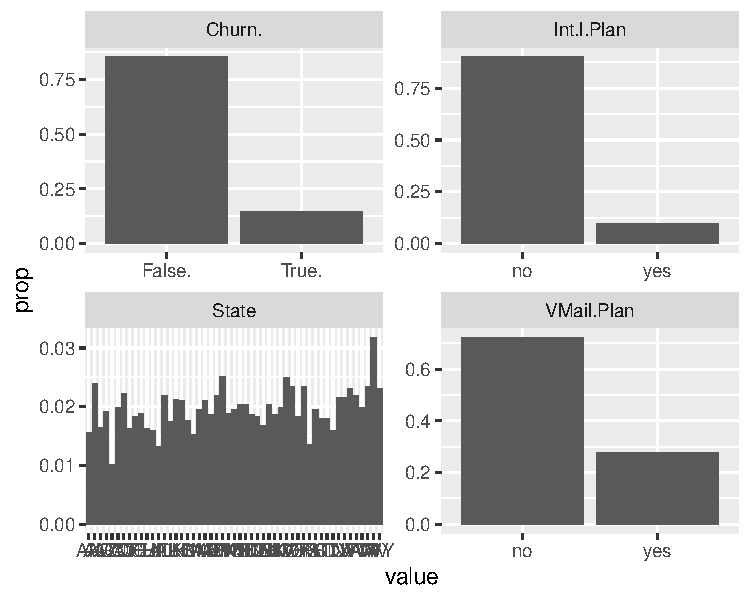
\includegraphics[width=\maxwidth]{figure/Overviews_plots-1} 

}


\begin{kframe}\begin{alltt}
\hlkwd{ggplot}\hlstd{(}\hlkwd{gather}\hlstd{(numerics),} \hlkwd{aes}\hlstd{(value))} \hlopt{+}
  \hlkwd{geom_histogram}\hlstd{()} \hlopt{+}
  \hlkwd{facet_wrap}\hlstd{(}\hlopt{~}\hlstd{key,} \hlkwc{scales}\hlstd{=}\hlstr{'free'}\hlstd{)}
\end{alltt}


{\ttfamily\noindent\itshape\color{messagecolor}{\#\# `stat\_bin()` using `bins = 30`. Pick better value with `binwidth`.}}\end{kframe}

{\centering 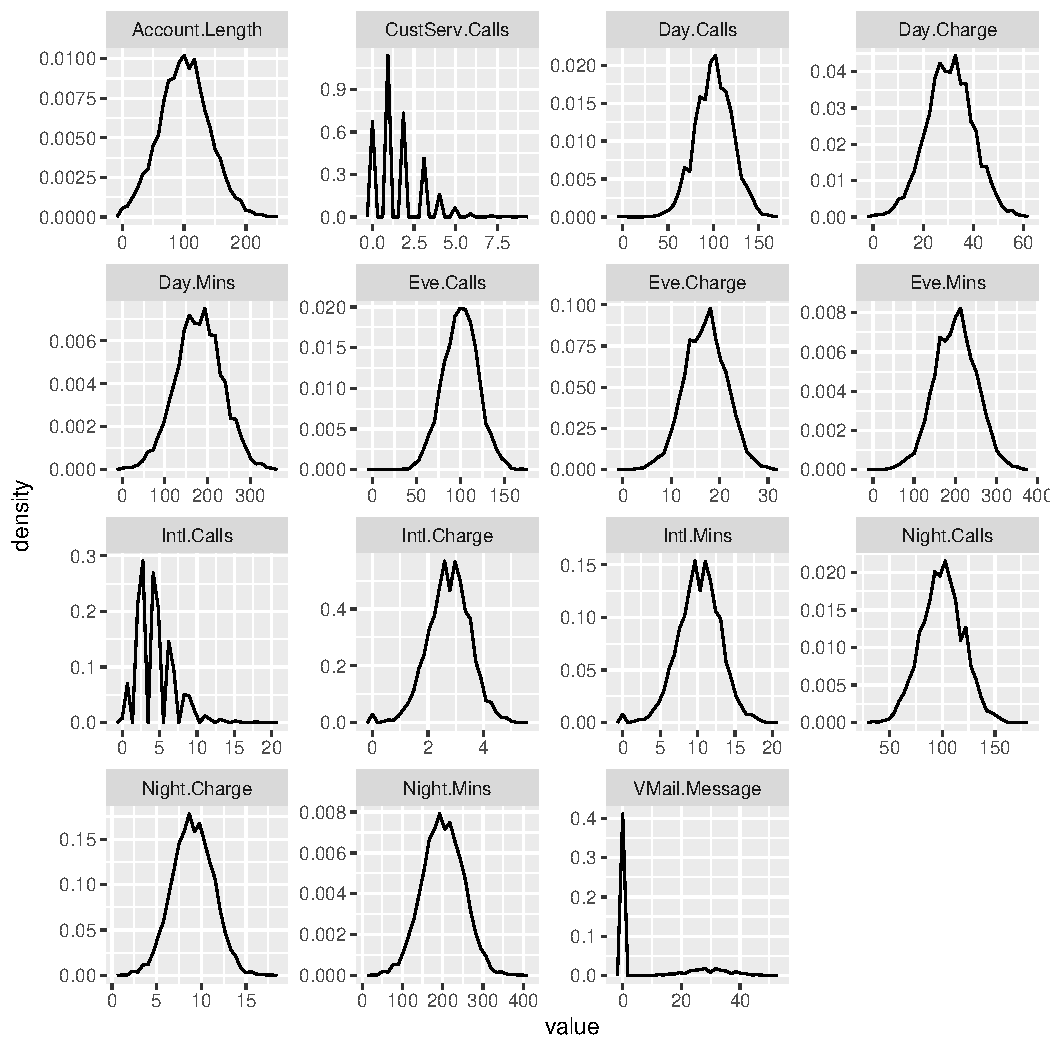
\includegraphics[width=\maxwidth]{figure/Overviews_plots-2} 

}


\begin{kframe}\begin{alltt}
\hlkwd{ggplot}\hlstd{(}\hlkwd{gather}\hlstd{(numerics),} \hlkwd{aes}\hlstd{(value))} \hlopt{+}
  \hlkwd{geom_boxplot}\hlstd{()} \hlopt{+}
  \hlkwd{facet_wrap}\hlstd{(}\hlopt{~}\hlstd{key,} \hlkwc{scales}\hlstd{=}\hlstr{'free'}\hlstd{)}
\end{alltt}
\end{kframe}

{\centering 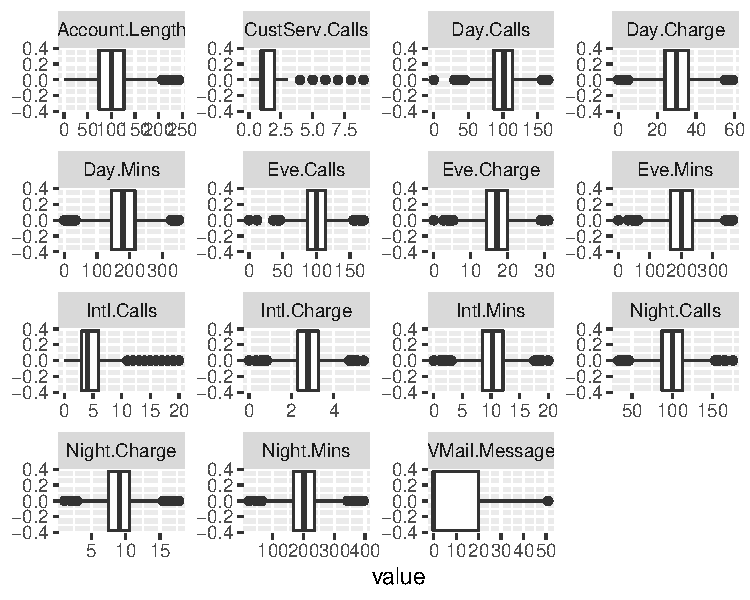
\includegraphics[width=\maxwidth]{figure/Overviews_plots-3} 

}



\end{knitrout}

\item{c)}

\begin{knitrout}
\definecolor{shadecolor}{rgb}{0.969, 0.969, 0.969}\color{fgcolor}\begin{kframe}
\begin{alltt}
\hlstd{continuous} \hlkwb{<-} \hlkwd{subset}\hlstd{(numerics,} \hlkwc{select}\hlstd{=}\hlkwd{sapply}\hlstd{(numerics,} \hlkwa{function}\hlstd{(}\hlkwc{x}\hlstd{)} \hlopt{!}\hlkwd{is.integer}\hlstd{(x)))}
\hlkwd{ggpairs}\hlstd{(continuous)}
\end{alltt}
\end{kframe}

{\centering 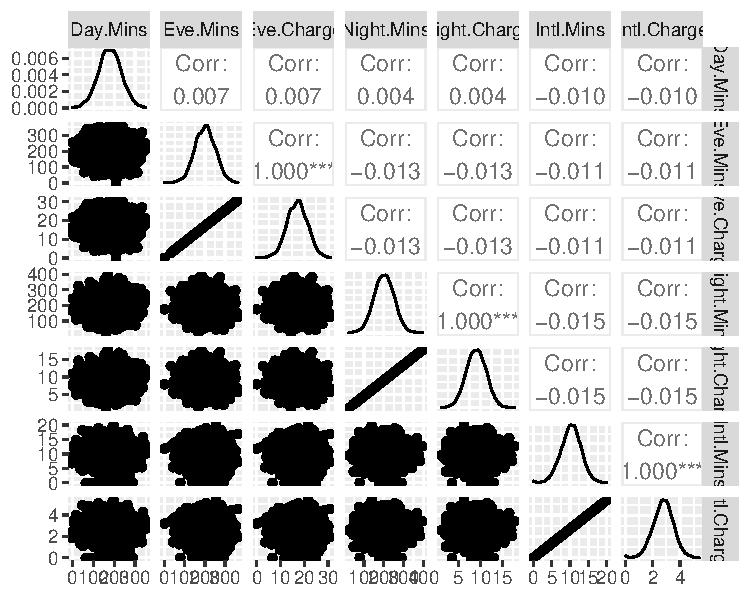
\includegraphics[width=\maxwidth]{figure/Pair_plot_for_continuous_variables-1} 

}



\end{knitrout}

\item{d)}

\begin{knitrout}
\definecolor{shadecolor}{rgb}{0.969, 0.969, 0.969}\color{fgcolor}\begin{kframe}
\begin{alltt}
\hlkwd{sapply}\hlstd{(numerics, range)}
\end{alltt}
\begin{verbatim}
##      Account.Length VMail.Message Day.Mins Day.Calls Day.Charge Eve.Mins
## [1,]              1             0      0.0         0          0      0.0
## [2,]            243            51    350.8       165         59    363.7
##      Eve.Calls Eve.Charge Night.Mins Night.Calls Night.Charge Intl.Mins
## [1,]         0       0.00       23.2          33         1.04         0
## [2,]       170      30.91      395.0         175        17.77        20
##      Intl.Calls Intl.Charge CustServ.Calls
## [1,]          0         0.0              0
## [2,]         20         5.4              9
\end{verbatim}
\end{kframe}
\end{knitrout}

\begin{knitrout}
\definecolor{shadecolor}{rgb}{0.969, 0.969, 0.969}\color{fgcolor}\begin{kframe}
\begin{alltt}
\hlkwd{sapply}\hlstd{(factors, levels)}
\end{alltt}
\begin{verbatim}
## $State
##  [1] "AK" "AL" "AR" "AZ" "CA" "CO" "CT" "DC" "DE" "FL" "GA" "HI" "IA" "ID" "IL"
## [16] "IN" "KS" "KY" "LA" "MA" "MD" "ME" "MI" "MN" "MO" "MS" "MT" "NC" "ND" "NE"
## [31] "NH" "NJ" "NM" "NV" "NY" "OH" "OK" "OR" "PA" "RI" "SC" "SD" "TN" "TX" "UT"
## [46] "VA" "VT" "WA" "WI" "WV" "WY"
## 
## $Area.Code
## [1] "408" "415" "510"
## 
## $Int.l.Plan
## [1] "no"  "yes"
## 
## $VMail.Plan
## [1] "no"  "yes"
## 
## $Churn.
## [1] "False." "True."
\end{verbatim}
\end{kframe}
\end{knitrout}

\begin{knitrout}
\definecolor{shadecolor}{rgb}{0.969, 0.969, 0.969}\color{fgcolor}\begin{kframe}
\begin{alltt}
\hlkwd{library}\hlstd{(moments)}
\hlkwd{sapply}\hlstd{(numerics, skewness)}
\end{alltt}
\begin{verbatim}
## Account.Length  VMail.Message       Day.Mins      Day.Calls     Day.Charge 
##    0.096562812    1.264254335   -0.029063980   -0.111736324   -0.027264807 
##       Eve.Mins      Eve.Calls     Eve.Charge     Night.Mins    Night.Calls 
##   -0.023866709   -0.055538130   -0.023847250    0.008917276    0.032484942 
##   Night.Charge      Intl.Mins     Intl.Calls    Intl.Charge CustServ.Calls 
##    0.008882237   -0.245025603    1.320883367   -0.245176105    1.090868260
\end{verbatim}
\end{kframe}
\end{knitrout}

\begin{knitrout}
\definecolor{shadecolor}{rgb}{0.969, 0.969, 0.969}\color{fgcolor}\begin{kframe}
\begin{alltt}
\hlstd{cv} \hlkwb{<-} \hlkwa{function}\hlstd{(}\hlkwc{X}\hlstd{)} \hlkwd{sd}\hlstd{(X)} \hlopt{/} \hlkwd{mean}\hlstd{(X)}

\hlkwd{sapply}\hlstd{(numerics, cv)}
\end{alltt}
\begin{verbatim}
## Account.Length  VMail.Message       Day.Mins      Day.Calls     Day.Charge 
##      0.3940255      1.6901282      0.3029752      0.1998203      0.3080191 
##       Eve.Mins      Eve.Calls     Eve.Charge     Night.Mins    Night.Calls 
##      0.2523324      0.1989988      0.2523287      0.2517715      0.1954755 
##   Night.Charge      Intl.Mins     Intl.Calls    Intl.Charge CustServ.Calls 
##      0.2517746      0.2727127      0.5494459      0.2726534      0.8417223
\end{verbatim}
\end{kframe}
\end{knitrout}

\end{description}

\section{Etap III}

\begin{description}

\item{a)}


\item{b)}

\end{description}

\end{document}
